\documentclass[man, noapacite]{apa2}

\usepackage{hyperref}
% \usepackage{pslatex}
\usepackage{pdfsync}
\usepackage{apacite2}
\usepackage{amsmath}
\usepackage{graphicx}
\usepackage{topcapt}
\usepackage{color}

% don't split footnotes
\interfootnotelinepenalty=10000

% comment command
\newcommand{\blue}[1]{\textcolor{blue}{#1}}
 
\title{Uninformative negation is infelicitous to both adults and children}

\author{Ann E. Nordmeyer and Michael C. Frank}
\affiliation{Department of Psychology, Stanford University}

\shorttitle{Contexts of negation}

\abstract{REVISE: Why  do  some  negative  sentences  sound  strange,  even  when they are both true and grammatical?  We explore the pragmatics of negation by examining adults� and children's explicit felicity judgments of negative sentences in context. In Experiments 1 and 2, we found that  a  pragmatically  supportive  context  elicited  higher  felicity ratings for negative sentences, and that negative sentences expressing nonexistence were rated higher than negative sentences referring to an alternative object.  A model of the informativeness of a sentence in context predicts our results, suggesting that the relative felicity of negation in context is due to general pragmatic principles rather than the conceptual difficulty of negation. In Experiment 3, we showed that children are also sensitive to the contexts of true negative sentences, suggesting that children also prefer negative sentences when they are produced in a more informative context.  We discuss the pragmatics  of  negation  in  light  of  these  results,  arguing  that both adults' and children's difficulty processing negation is due to changes in the informativeness, and thus the felicity, of these sentences in different contexts.}  

\begin{document}
\maketitle


\section{Introduction}

A sentence that is both grammatical and true can nevertheless sound odd in some contexts. If you open a mysterious box and find that it is empty, it's weird to say ``This box doesn't have any chocolates in it,'' despite the truth of the proposition. But the same sentence becomes perfectly reasonable if you are in a chocolate store surrounded by boxes filled with chocolate.  What is it about context that makes some sentences sound strange (\emph{infelicitous}) in one situation, but normal in another?  

Theories of pragmatics attempt to provide an account of how language users move from the literal semantics of a sentence to an inference about the speaker's intended meaning. For example, according to Grice's \citeyear{grice1975} Cooperative Principle, speakers should produce utterances that are truthful, relevant, and informative.  By assuming that speakers do so, listeners can make inferences about intended meaning that go beyond the sentence's literal meaning. Modern neo-Gricean theories tend to derive such inferences from the tension between being informative with respect to a communicative goal and minimizing the effort expended \cite{horn1984,levinson2000,frank2012}. These theories make predictions about sentence felicity: As in our example above, a sentence that is not pragmatically supported can sound strange even when it is both grammatical and true.  Here, we argue that both adults' and children's difficulty processing negative sentences can be explained by this relationship between contextual pragmatics and felicity.

\subsection{The role of context in the processing of negation}

Negative sentences can be difficult to process, even for adults.  When presented without any context, people take longer to evaluate the truth of negative sentences such as ``star isn't above plus'' compared to positive sentences \cite{hclark1972, carpenter1975, just1971, just1976}.  Similarly, in EEG studies, participants who read true negative sentences like ``A bird is not a truck'' show a similar N400 response (a negative waveform that responds to semantically unexpected stimuli) as a corresponding false positive sentence like ``A bird is a truck'' \cite{fischler1983, ludtke2008}.  Based on these findings, it has been suggested that there is something specific to the representation of negation that makes processing negative sentences so challenging.

As our original example demonstrates, however, negative sentences are particularly sensitive to the effects of context.    In a classic study, \citeNP{wason1965} found that when participants were asked to describe an array of e.g. seven red dots and one blue dot, participants who described the stimuli in terms of an exception to a rule (e.g. ``Circle number four is blue and the rest are red'') were faster to process true negative sentences compared to participants who described the stimuli in other ways (e.g. ``Seven circles are red and one is blue'').  Similarly, supportive written contexts, such as a narrative framing where the negated feature is made salient prior to reading the negative sentence, can facilitate the processing of negation \cite{glenberg1999, ludtke2006, nieuwland2008, dale2011}, and reduce the N400 response to true negative sentences \cite{nieuwland2008}.  Although these findings suggest that context can have a powerful effect on the processing of negative sentences, it is not clear what mechanism leads to this facilitative effect.  

One possible mechanism is that general pragmatic principles can explain the both the processing cost of negation and the supportive effect of context.  In recent work (Nordmeyer \& Frank, under review), we demonstrated a graded effect of context on the processing of negation, with negative sentences processed faster as the base rate of the negated feature increased.  Specifically, negative sentences that were more relevant and informative given the context were processed faster.  We found that this effect of context could be reliably predicted by the probability of a speaker using the same sentence to describe the same picture.  Speakers are unlikely to produce sentences that are uninformative and irrelevant, and correspondingly listeners take longer to respond to unlikely sentences.  

Previous work has linked reaction time to syntactic surprisal, an information-theoretic measure predicting that low-probability utterances will be processed slower than high-probability utterances \cite{levy2008}.  If \emph{pragmatic surprisal}---the probability of an utterance being produced given the context---is responsible for the context effects seen in negation processing, these context effects should be reflected in adults' explicit felicity judgments as well, with more informative sentences eliciting higher felicity ratings than less informative sentences.  This finding would lend further support to our hypothesis that the effects of context on negative sentences are due to pragmatic principles that govern communication more generally, rather than some unique effect of negation. 


\subsection{Children's understanding of negation}

There is a puzzle in children's acquisition of negation: Although children begin producing negation spontaneously and accurately before age two \cite{bloom1973, pea1980, pea1982}, preschoolers struggle to respond correctly to true negative sentences.  For example, the majority of three-year-olds and nearly half of four- and five-year-olds classified true negative sentences as ``wrong'' when, for example, an experimenter pointed to an apple and said ``this is not a banana'' \cite{kim1985}, despite the fact that they had no difficultly classifying true and false positive sentences.   This finding, along with others \cite{gilkerson2005, loder2008, nordmeyer2014b}, suggests that children struggle to process negative sentences, despite the fact that they produce them so early.  

One possible solution to this puzzle is that children are behaving rationally based on a Gricean view of communication.  In most experiments of children's comprehension of negation, such as the one described above, children hear negative sentences without any supportive pragmatic context.  In these contexts, although the sentences are not \emph{false}, they are perhaps \emph{wrong} according the the Cooperative Principle.  In contrast, studies that have elicited spontaneous negations from children tend to use familiar contexts, such as reading picture books in an interactive, game-like setting \cite{pea1982, hummer1993}.  When children hear a true negative sentence and indicate that it is ``wrong'' \cite<e.g.>{kim1985}, they may be reacting to the infelicity of the sentence rather than its truth value.  

If the effect of context on negation is primarily pragmatic in nature, we can use negation as a case study to explore children's sensitivity to contextual pragmatics.  Evidence is mixed regarding whether children are sensitive to Gricean pragmatic principles.  Some data suggest that children struggle to make scalar implicatures; for example, accepting a sentence like ``Some of the horses jumped over the fence'' in a scenario where \emph{all} of the horses had jumped over the fence (\citeNP{papagragou2003}, see also \citeNP{noveck2001}) .  Other evidence, however, suggests that children are sensitive to pragmatics and can make pragmatic inferences in a number of domains such as contextually-based implicatures \cite{papafragou2004, barner2011, yoon2015, stiller2015}, adjective use \cite{horowitz2012, horowitz2014}, and epistemic states \cite{hochstein2014}.  By examining children's judgments of negative sentences in different contexts, we can ask whether children's aforementioned difficulty with negation is actually due to an awareness that the same sentence can be a ``good'' thing to say in one context, but a ``silly'' thing to say in another.

\subsection{The current study}

In this paper we explore the effect of context on the explicit sentence felicity judgments of adults and children.  We operationalize context as information that influences expectations about an upcoming utterance.   In natural contexts, the information that constitutes ``context'' could include visual information, words, or actions in the setting of a conversation or another shared task \citeA{clark1996}.  In our experiments, we use visual contexts in which we manipulate the base rate of certain features in the stimuli.  For example, in a context where three people have apples and one person does not, it feels very natural to describe the last person by saying ``He doesn't have apples.''  In contrast, in a context where no one is holding any objects (i.e. there are no apples present anywhere), the same sentence is uninformative, because it could refer to any of the people in the scene, and there is no reason to discuss apples.  In Experiments 1 and 2, we find that adults rate sentences in the former context as more felicitous than sentences in the latter context, supporting the findings of past research in the domain of sentence processing \cite{nordmeyer2014}.  

We hypothesize that the effects of context on the felicity of negative sentences is driven primarily by Neo-Gricean pragmatic principles.  To formalize this prediction, we compare the results of our adult data in Experiments 1 and 2 to the predictions of a Rational Speech Act model \cite{frank2012}, which predicts that listeners expect speakers to produce maximally informative utterances. In the above examples, the RSA model predicts that the sentence ``he doesn't have apples'' is more informative -- and therefore more likely to be produced -- in the context where everyone else has apples, compared to the context where no one has apples, because in this context the utterance uniquely identifies the referent of the sentence.  We find that sentences that are more probable according to this model are rated as more felicitous by our participants.  

In Experiment 3, we examine whether preschoolers are sensitive to the contexts of negative sentences.  If children's difficulty comprehending negative sentences is due to conceptual complexity or an undeveloped semantic understanding of negation, then these children should rate true negative sentences as bad regardless of the context in which they occur.  If, however, children are actually rating true negative sentences as ``wrong'' because of the infelicity of pragmatically unsupported negation, then we should see children's performance improve when they are asked to rate true negative sentences in a supportive, informative context.  We find evidence for the latter hypothesis, suggesting that children's difficulty understanding negative sentences on classic tests of comprehension is due to pragmatic sensitivity rather than a failure to process negation.

The results of past research on negation suggest a paradox: Negative sentences are produced early by children and frequently throughout adulthood, yet both adults and children appear to find negation difficult on tasks that test their processing and comprehension.  Our data suggest that the difficulty of negative sentences is due primarily to the infelicity of negative sentences in unsupported contexts, rather than any representational or syntactic difficulty specific to negation.  Negative sentences are more likely to violate the Cooperative Principle, because a negative sentence can refer truthfully to a broader set of referents (e.g. at any given moment, there are more people in the world who are \emph{not} holding apples than people who \emph{are} holding apples, more boxes that do \emph{not} contain chocolate than boxes that \emph{do} contain chocolate, etc.), making negative sentences less informative by default.  In the right contexts, however, negative sentences can be just as informative as positive sentences, suggesting that the ``difficulty'' of negation is actually due to a general difficulty understanding unlikely and therefore infelicitous utterances.

\section{Experiment 1}

In Experiment 1, we focused on two possible referents of negation.  The same negative sentence can refer to the absence of a feature (nonexistence) or to an alternative feature (alternative).  For example, the sentence ``This box doesn't contain chocolate'' might refer to an empty box (e.g. nonexistence) or a box containing an alternative object (e.g. broccoli instead of chocolate).  Previous work suggests that adults are faster to identify the referent of nonexistence compared with alternative negation \cite{nordmeyer2013, nordmeyer2014b}.  This finding could be due to processing demands (e.g. identifying a missing feature is easier than identifying a changed feature), but it could also reflect an expectation about the pragmatics of negation; adults may find alternative negation infelicitous because they expect the sentence to describe present, rather than absent, features.  

Experiment 1 explored how different contexts affected participants' felicity ratings for negative sentences.  Half of the participants in Experiment 1 saw sentences presented in a context where none of the surrounding characters had any objects on their table (the \emph{none} condition), and the other half saw sentences presented in a context where everyone except for the target character possessed the negated object, e.g. apples (the \emph{target} condition).  In half of the true negative trials, the referent of the negative sentence was a character who had nothing (nonexistence negation).  In the other half of true negative trials, the referent of the sentence was a character who had some other object, e.g. a cat (alternative negation).  Finally, we examined how different syntactic framings might influence sentence judgments (e.g. ``has no apples'' and ``doesn't have apples''). If the facilitative effect of context on negation driven by the informativeness of negative sentences in different contexts, then these same effects should appear regardless of the syntactic framing of the sentences.  

\subsection{Method}

\subsubsection{Participants}

We recruited a planned sample of 100 adults to participate in an online experiment through Amazon Mechanical Turk; six participants were excluded for indicating that they were under 18 after completing the experiment, and two participants who did not list English as their native language were excluded.  Of the remaining 92 participants, 40 were male and 40 were female, three declined to report gender, and ages ranged from 18 -- 65+.  We restricted participation to individuals in the United States and paid 35 cents for the experiment, which took approximately five minutes to complete.  Participants were randomly assigned to either the \emph{none} condition (n=47) or the \emph{target} condition (n=45).  


\subsubsection{Stimuli}

We created 16 trial items. On each trial, four Sesame Street characters were shown standing behind tables.  One character was randomly selected as the ``target'' character, designated by a red box (see Figure \ref{fig:trial}). The remaining three characters were designated as ``context'' characters.


\begin{figure}[t]
\begin{center} 
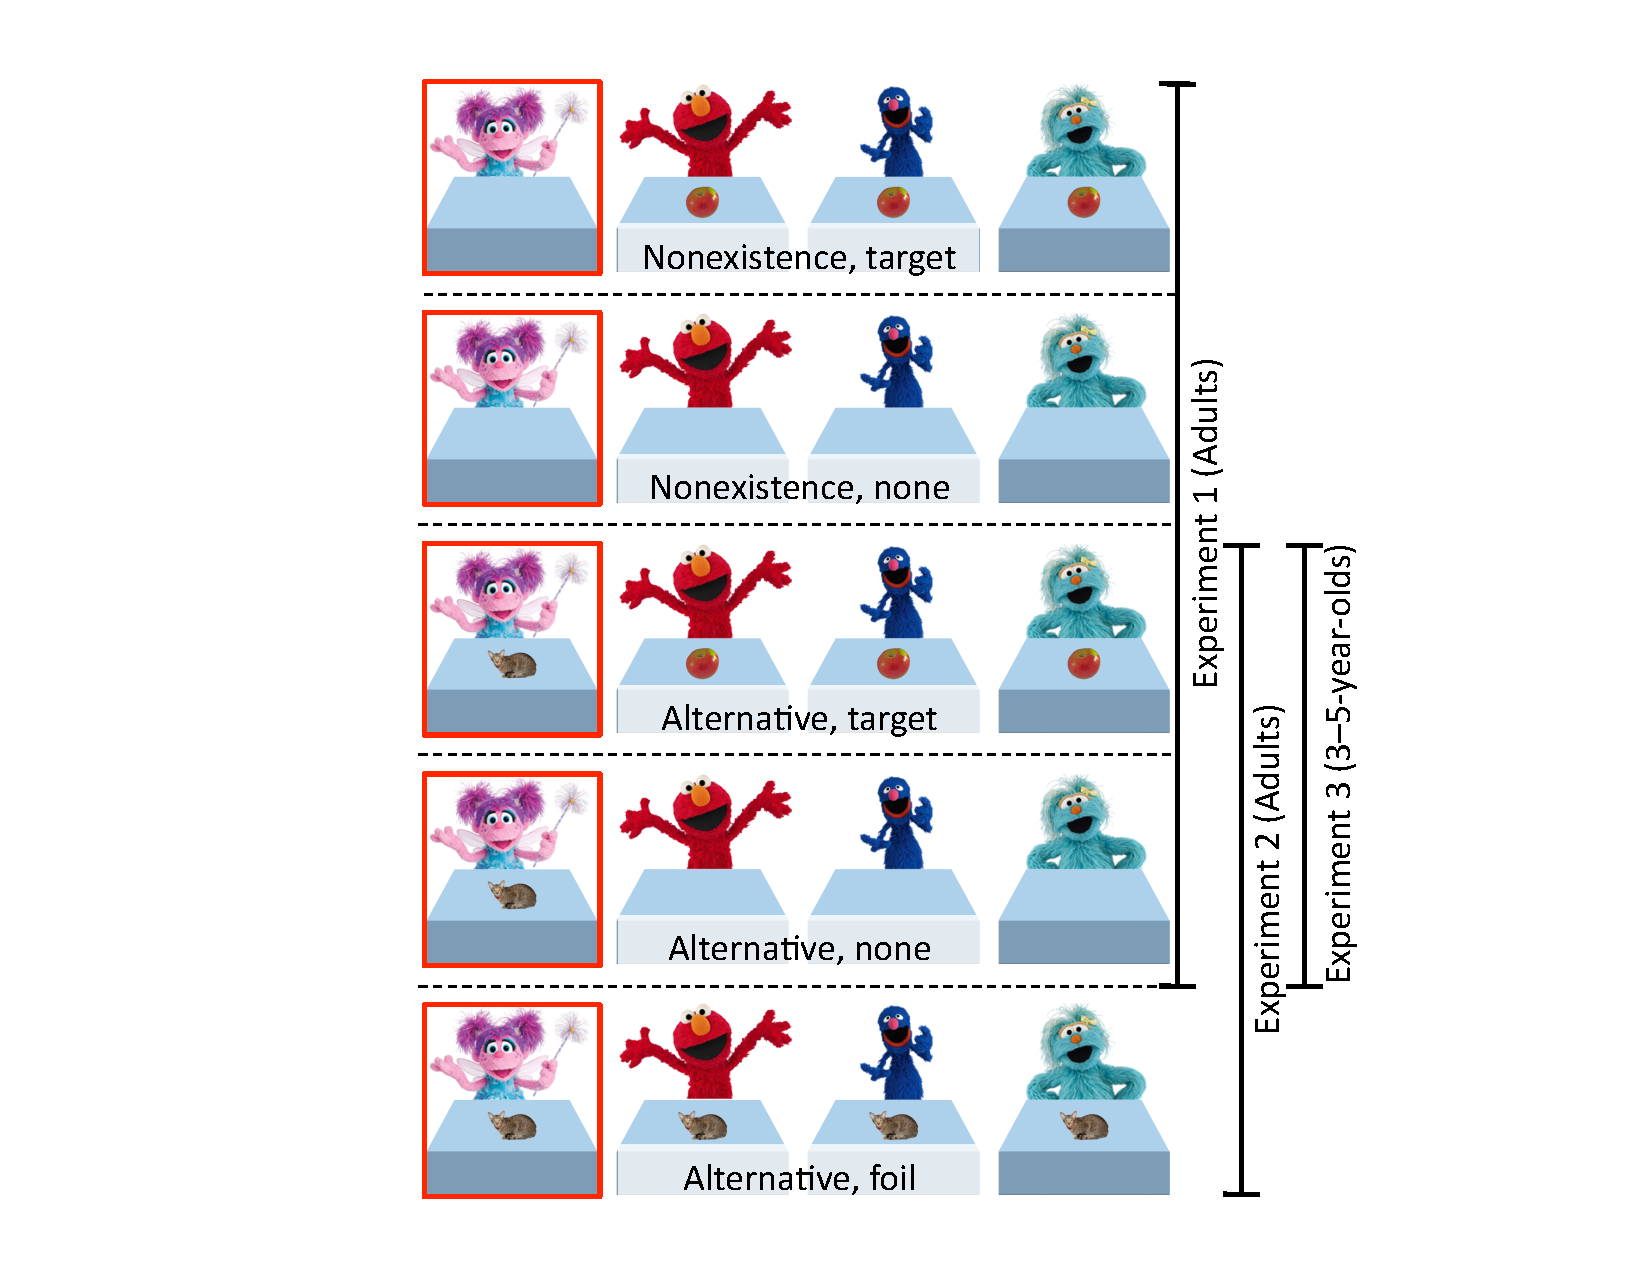
\includegraphics[width=3in]{figures/trialtypes.pdf}
\caption{\label{fig:trial} The five types of true negative trials across Experiment 1 and Experiment 2.  In this example, the target object is an apple and the alternative object is a cat. Below each set of pictures a sentence appeared about the character in red, e.g. ``Abby doesn't have an apple.''}  
\end{center} 
\end{figure}

Participants were randomly assigned to the \emph{none} context condition or the \emph{target} context condition.  In the \emph{none} condition, the context characters all stood behind empty tables.  In the \emph{target} condition, each context character had an identical object on their table.  The objects belonged to one of four categories: animals (cat, dog, horse cow), vehicles (car, bus, boat, truck), food (apple, banana, cookie, orange), and household objects (fork, spoon, bowl, plate).  Stimuli were created using images from the Bank of Standardized Stimuli \cite{brodeur2010}.  

Below the characters was a sentence about the target character.  Across the entire experiment, six of these sentences were positive sentences such as ``[character] has a/an [object].''  Five were negative sentences of the form ``[character] has no [object]'' and five were negative sentences of the form ``[character] doesn't have a/an [object].'' 

The target character had a target object, an alternative object (``alternative'' trials), or nothing (``nonexistence'' trials), allowing us to examine two different negative concepts (see Figure \ref{fig:trial} for depictions of these trials and the different context conditions).    Trial conditions were crossed such that each participant saw six true positive trials, two false positive trials (one alternative and one nonexistence), two false negative trials (one ``has no'' sentence type and one ``doesn't have'' sentence type), and eight true negative trials (two ``has no''/nonexistence, two ``has no''/alternative, two ``doesn't have/nonexistence'', and two ``doesn't have/alternative'').  Each of these trial types was randomly assigned to a target object, and trials were presented in a random order.  

A slider bar was positioned beneath the sentence, with a seven-point scale ranging from ``Very Bad'' to ``Very Good.''  A progress bar at the top of the screen informed participants how much of the experiment they had completed. 

\subsubsection{Procedure}

Participants first saw an instructions screen that briefly described the task and informed them that they could stop at any time.  Once participants agreed to participate, they saw an instructions screen that explained the task in more detail.  Participants were asked to rate how ``good'' each sentence was based on how a hypothetical speaker might behave, e.g. ``if no one would ever say a particular sentence in this context, or if it is just wrong, rank that as `Very Bad,' but if something is right and sounds perfectly normal, mark it as `Very Good.''' Participants were encouraged to use the entire scale. On each trial the pictures, sentence, and slider bar appeared simultaneously, and participants had to make a selection on the scale in order to progress to the next trial.  The experiment can be viewed 

\subsection{Results and Discussion}

NOTE: Is this table of means too much?  There are so many different trial types in this experiment.  In the table I changed the phrase "negation type" to "referent type" because "negation type" doesn't make sense for the false positive trials (really what I mean is, does the sentence refer to someone with nothing or someone with some other object); I will probably make this change throughout if it seems sensible to you.  I spent a while thinking about the best way to organize this table; I'm not sure this is the best option.  Also, I ended up leaving the analysis with just true negative sentences...this is mostly because the graph with false sentences ends up just looking like a huge waste of space because the false negs are at floor and show no context effects.  Could I present a model of all negative sentences, and just plot the true negative means?

Participants treated the scale as expected, consistently rating true sentences much higher than false sentences.   Furthermore, participants consistently rated positive sentences higher than negative sentences.  There was no effect of context, syntactic frame, or referent type on true positive sentences, false positive sentences, or false negative sentences, likely due to a ceiling effect for true positive sentences and a floor effect for false sentences (see Table \ref{fig:m1}). 

Focusing on true negative sentences, these sentences were rated significantly higher in a \emph{target} context compared to a \emph{none} context. For example, the sentence ``Abby has no apples'' was rated higher when all of the other characters \emph{had} apples, compared to contexts where all of the other characters had nothing. This finding supports our hypotheses and replicates patterns previously seen in studies of processing time using explicit felicity judgments.  Negative sentences expressing nonexistence were rated as more felicitous than negative sentences referring to an alternative object (see Figure \ref{fig:s1}). 

\begin{table}[t]
\caption{\label{tab:m1} Mean felicity rating for different trial types in Experiment 1, based on ratings given on a 7-point scale.}
\begin{center}
\small\addtolength{\tabcolsep}{-5pt}
\begin{tabular}{llllrr}
  \hline
  Context & Sentence type & Truth Value & Referent Type & Mean & Std. Dev. \\ 
  \hline
  None & Positive (``has X'') & True & Target item & 6.51 & 0.89\\ 
  None & Positive (``has X'') & False & Nothing & 2.51 & 1.94\\ 
  None & Positive (``has X'') & False & Alternative item & 2.04 & 1.82\\ 
  None & Negative (``doesn't have X'') & True & Nothing & 5.29 & 1.44\\ 
  None & Negative (``doesn't have X'') & True & Alternative item & 4.83 & 1.92\\ 
  None & Negative (``doesn't have X'') & False & Target item & 2.00 & 1.64\\ 
  None & Negative (``has no X'') & True & Nothing & 4.78 & 1.68\\ 
  None & Negative (``has no X'')  & True & Alternative item & 4.15 & 1.78\\ 
  None & Negative (``has no X'') & False & Target item & 1.40 & 0.77\\ 
  Target & Positive (``has X'') & True & Target item & 6.42 & 0.76\\ 
  Target& Positive (``has X'') & False & Nothing & 1.88 & 1.47\\ 
  Target & Positive (``has X'') & False & Alternative item & 1.83 & 1.73\\ 
  Target & Negative (``doesn't have X'') & True & Nothing & 6.34 & 1.11\\ 
  Target & Negative (``doesn't have X'') & True & Alternative item & 5.74 & 1.41\\ 
  Target & Negative (``doesn't have X'') & False & Target item & 1.89 & 1.60\\ 
  Target & Negative (``has no X'') & True & Nothing & 5.61 & 1.51\\ 
  Target & Negative (``has no X'')  & True & Alternative item & 4.96 & 1.41\\ 
  Target & Negative (``has no X'') & False & Target item & 1.58 & 0.99\\ 
   \hline
\end{tabular}
\end{center}
\end{table}

To test the reliability of these findings, we fit a linear mixed-effects model examining the interaction between context, negation type (e.g. nonexistence or alternative), and negation framing (e.g. ``has no X'' vs. ``doesn't have X'') on felicity ratings.\footnote{ The model specification was as follows: \texttt{rating $\sim$ context~$\times$~negation type~$\times$~negation frame + (negation type~$\times$~negation frame~\textbar~subject) +  (negation type~$\times$~negation frame~\textbar~item)}.  Significance was calculated using the standard normal approximation to the $t$ distribution \cite{barr2013}. Data and analysis code can be found at \href{http://github.com/anordmey/cogsci15}{http://github.com/anordmey/cogsci15}.}  Because we were primarily interested in the effects of context on true negative sentences, we focused on these trials in our analyses, though the effects reported here are significant in full models of all sentence types as well.

Examining the model, we found a main effect of context, with true negative sentences presented in a \emph{target} context eliciting significantly higher ratings than true negative sentences presented in a \emph{none} context ($\beta= 1.08$, $p< .001$).  We found main effects of negation type, with alternative negation receiving lower ratings than nonexistence negation ($\beta= -.43$, $p< .05$), as well as a marginally significant effect of negation framing, with sentences of the form ``has no X'' receiving lower ratings than sentences of the form ``doesn't have X''  ($\beta= -.49$, $p= .052$).  There were no interactions between negation frame, negation type, and context.  

Participants showed a slight preference for negative sentences with the framing ``doesn't have X'' over ``has no X''.  This preference did not interact with context or negation type; participants preferred the ``doesn't have'' framing for both alternative negation and nonexistence negation, and rated both sentence frames higher when they were presented in a \emph{target} context.  This finding suggests that effects of context on the felicity of negative sentences are not due to features of a specific syntactic frame.

In previous work we found that adults were somewhat faster to look at the referent of nonexistence negation compared with alternative negation \cite{nordmeyer2014b}. In that experiment, the difference between nonexistence and alternative negation could have arisen because of superficial, stimulus-level differences (i.e. it might be easier to identify a character with nothing than one with an alternative object). Our replication of this result using explicit felicity judgments suggests that this difference could result from pragmatic factors as well. One explanation for participants' preference for nonexistence negation is that a sentence such as ``Abby doesn't have an apple'' is more informative when Abby has nothing compared to when she has an alternative object.  In a strong context (e.g. one where everyone else has apples), using negation to point out Abby's lack of apples is informative because it uniquely identifies her character in the array.  When Abby has some alternative object (e.g. a cat), however, there is a \emph{more} informative utterance that a speaker could use (e.g. ``Abby has a cat'').  The existence of a more informative utterance makes these negative sentences less felicitous, even when they appear in context.

Overall, we found that a pragmatic context increases the felicity judgments of negative sentences.  Across all types of negation, participants assigned higher ratings to sentences that were presented with a \emph{target} context compared to sentences that were presented with a \emph{none} context.  This corroborates previous work in which more informative negative sentences were processed faster than less informative negative sentences \cite{nordmeyer2014}.  In the next section, we expand on this finding by testing the same sentences in a new context designed to test alternative possibilities for how context affects the pragmatics of negative sentences.

\begin{figure}
\begin{center} 
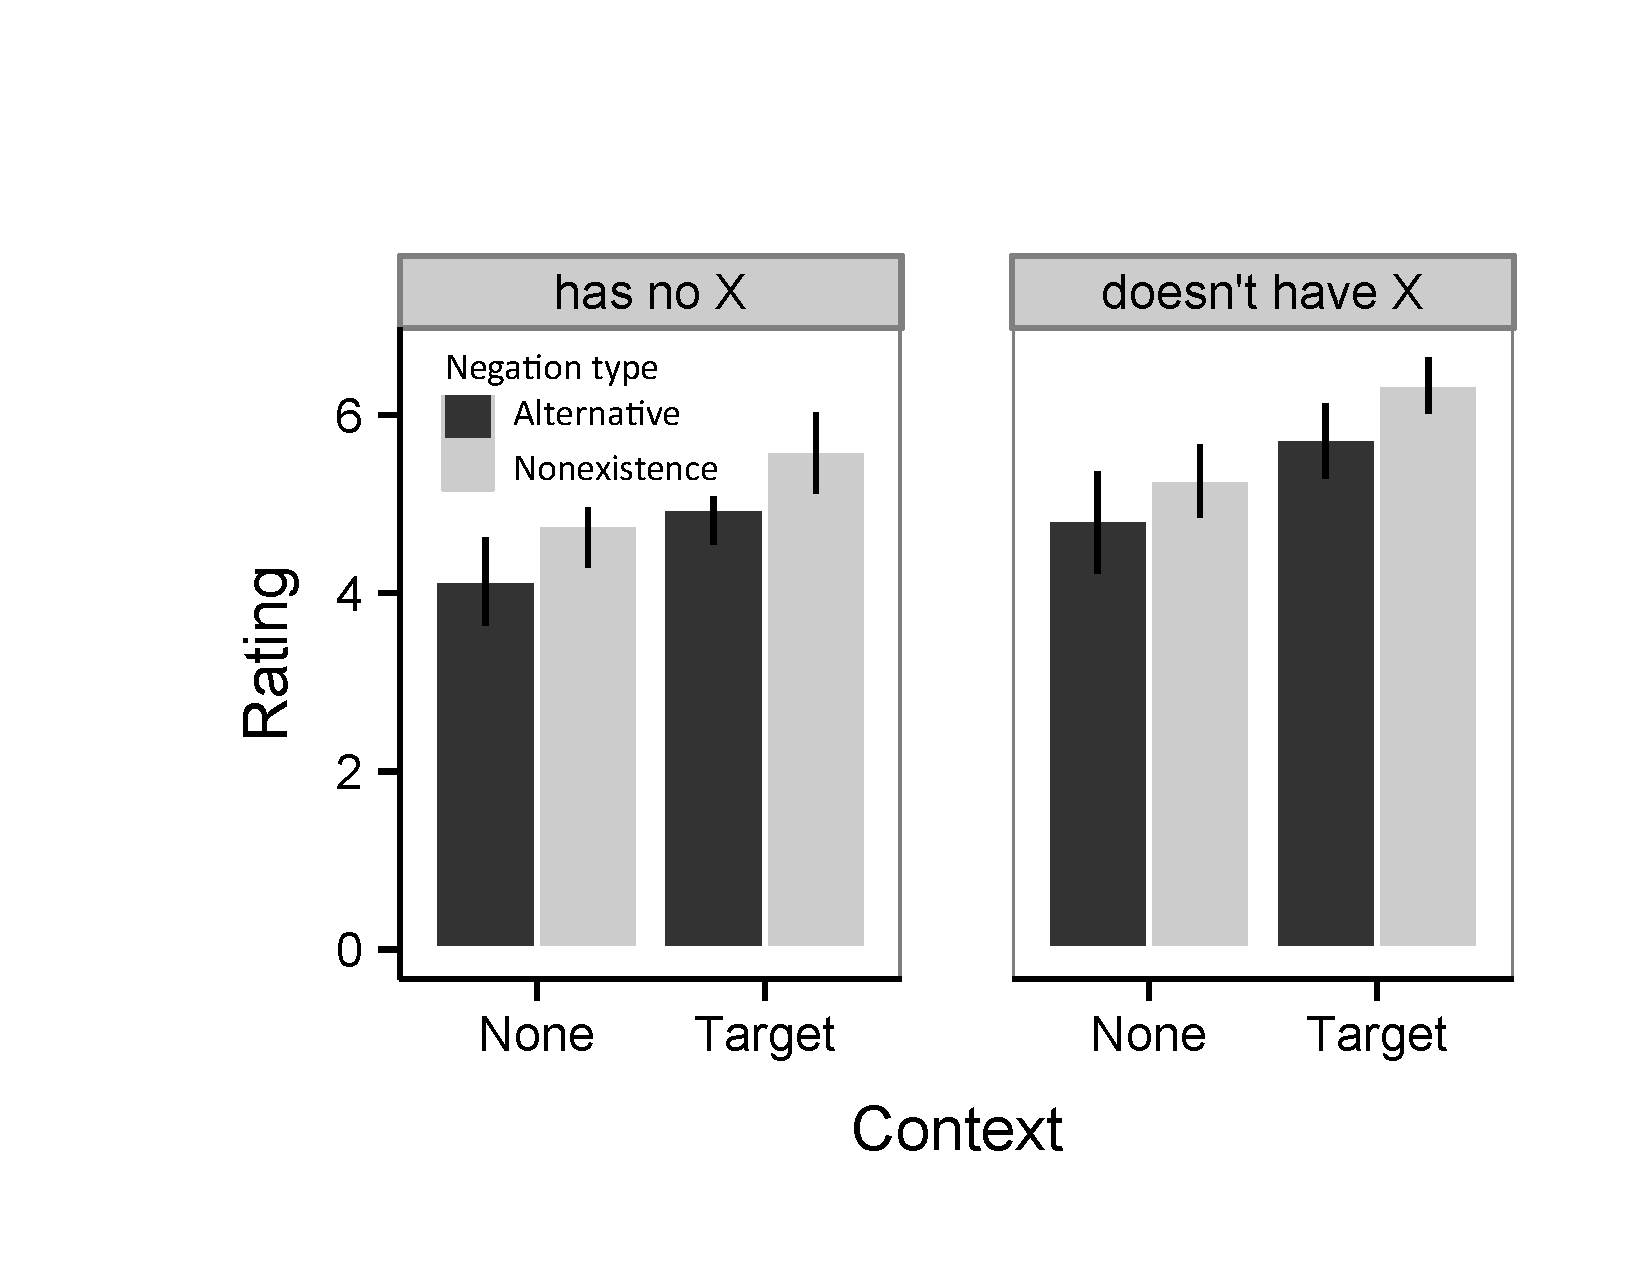
\includegraphics[width=3.25in]{figures/study1.pdf}
\caption{\label{fig:s1} Ratings for different types of true negative sentences in Experiment 1.  Sentences of the form ``...has no X'' are shown on the left, and sentences of the form ``...doesn't have X'' are shown on the right.  Negative sentences referring to an alternative object are shown in black, and negative sentences expressing nonexistence are shown in gray.  Error bars show 95\% confidence intervals.}
\vspace{-1.45cm}
\end{center} 
\end{figure}

\begin{table}[t]
\caption{\label{tab:s1} Coefficient estimates from a mixed-effects model predicting true negative sentence ratings in Experiment 1.}
\begin{center}
\small\addtolength{\tabcolsep}{-5pt}
\begin{tabular}{rrrr}
  \hline
 & Coefficient & Std. err. & t value \\ 
  \hline
(Intercept) & 5.28 & 0.19 & 27.16 \\ 
  Context (context) & 1.08 & 0.27 & 4.04  \\ 
  Negation type (alternative) & -0.43 & 0.17 & -2.50 \\
  Frame (``has no'') & -0.49 & 0.25 & -1.94 \\ 
  Context $\times$Negation type & -0.21 & 0.23 & -.92 \\
  Context $\times$Frame & -0.26 & 0.34 & -0.77 \\
  Negation type$\times$Frame & -0.22 & 0.23 & -0.94 \\
  Context$\times$Negation type$\times$Frame & 0.22 & 0.32 & 0.67 \\
   \hline
\end{tabular}
\end{center}
\end{table}

\section{Experiment 2}

In Experiment 2, we examined the effect of three contexts on alternative negation: A \emph{target} context, in which all context characters had the negated target object (identical to Experiment 1), a \emph{none} context, in which none of the context characters had any objects (identical to Experiment 1), and a \emph{foil} context, in which all context characters had an alternative object (e.g. a different object than the one negated in the negative sentences; see Figure \ref{fig:trial}).  Participants saw all three context conditions throughout the experiment, allowing us to examine within-subject effects of context.  

The addition of the ``foil'' context allowed us to test two competing hypotheses about the pragmatics of negation.  In true negative trials with a \emph{foil} context, all characters had the same objects on their table (e.g. cats), and the negative sentence referred to a different object (e.g. ``Abby doesn't have apples'').  Some previous work suggests that a critical element of the effect of context on negative sentences is the fact that the referent of the negative sentence is the ``odd one out'' \cite{wason1965}.  If this is the case, the \emph{foil} context might be even worse than the \emph{none} context, because the target of the negative sentence does not stand out from the context.  If, however, the effect of context is driven by the informativeness of negation, then there should be no difference between the \emph{foil} and \emph{none} contexts, because negative sentences are no less informative in the \emph{foil} context.  

%We also expected to replicate the same difference between the \emph{none} context and the \emph{target} context as was seen in Experiment 1: Negative sentences presented in a \emph{target} context should receive higher ratings than negative sentences presented in a \emph{none} context.  

\subsection{Method}

\subsubsection{Participants}

We recruited a planned sample of 200 adults to participate in an online experiment through Amazon Mechanical Turk.  We excluded from our analysis six participants who indicated that they were under 18 after completing the experiment, four participants who did not list English as their native language, and six participants who had participated in a previous version of the experiment.  Of the remaining 184 participants, 109 were mail and 72 were female, three declined to report gender, and ages ranged from 18 -- 65+.  We restricted participation to individuals in the United States and paid 40 cents for the experiment, which took approximately seven minutes to complete.  

\subsubsection{Stimuli}

Trials in Experiment 2 had the same structure as trials in Experiment 1, with a small set of exceptions. First, there were 24 trials. Second, all negative sentences were of the form ``[character] doesn't have a/an [object].'' Third, on each trial, the target character either had a target object on their table, or had an alternative object (eliminating the nonexistence trials).  Each participant evaluated nine true positive sentences, three false positive, three false negative, and nine true negative trials.

In Experiment 2, context was a within-subjects factor with three levels. In the \emph{none} context, context characters had nothing on their table, identical to the \emph{none} context condition in Experiment 1. In the \emph{target} context, context characters each had a target object on their table, same as the \emph{target} context condition in Experiment 1. In the \emph{foil} context, context characters had an alternative object on their table (e.g., all characters have a cat, but the sentence is about the presence/absence of apples; see Figure \ref{fig:trial}).  Each context condition appeared an equal number of times within each trial type.  

\subsubsection{Procedure}

The procedure was identical to Experiment 1.

\subsection{Results and Discussion}

As in Experiment 1, participants rated true sentences much higher than false sentences, and consistently rated  positive sentences somewhat higher than negative sentences.  As before, context did not affect ratings for true positive sentences or false sentences (see Table \ref{m2}).  True negative sentences were rated significantly higher when they were presented in a \emph{target} context compared to either the \emph{none} context or the \emph{foil} context (Figure \ref{fig:s2}).  There was no difference between sentences presented in a \emph{foil} context and sentences presented in a \emph{none} context.  

\begin{table}[t]
\caption{\label{tab:m2} Mean felicity rating for different trial types in Experiment 2, based on ratings given on a 7-point scale.}
\begin{center}
\small\addtolength{\tabcolsep}{-5pt}
\begin{tabular}{lllrr}
  \hline
  Context & Sentence type & Truth Value &  Mean & Std. Dev. \\ 
  \hline
  None & Positive & True & 6.68  & 0.54\\ 
  None & Positive & False &  1.62 & 1.32\\ 
  None & Negative & True &  5.31 & 1.52 \\ 
  None & Negative & False & 1.74  &1.55 \\ 
  Foil & Positive & True & 6.63  & 0.59\\ 
  Foil & Positive & False & 1.73  & 1.52\\ 
  Foil & Negative & True &  5.40 & 1.42 \\ 
  Foil & Negative & False & 1.70  & 1.49\\ 
  Target & Positive & True &  6.61 & 0.64 \\ 
  Target & Positive & False & 1.72  & 1.53 \\ 
  Target & Negative & True & 6.01  & 1.09 \\ 
  Target & Negative & False & 1.71  & 1.44\\ 
   \hline
\end{tabular}
\end{center}
\end{table}

\begin{figure}
\begin{center} 
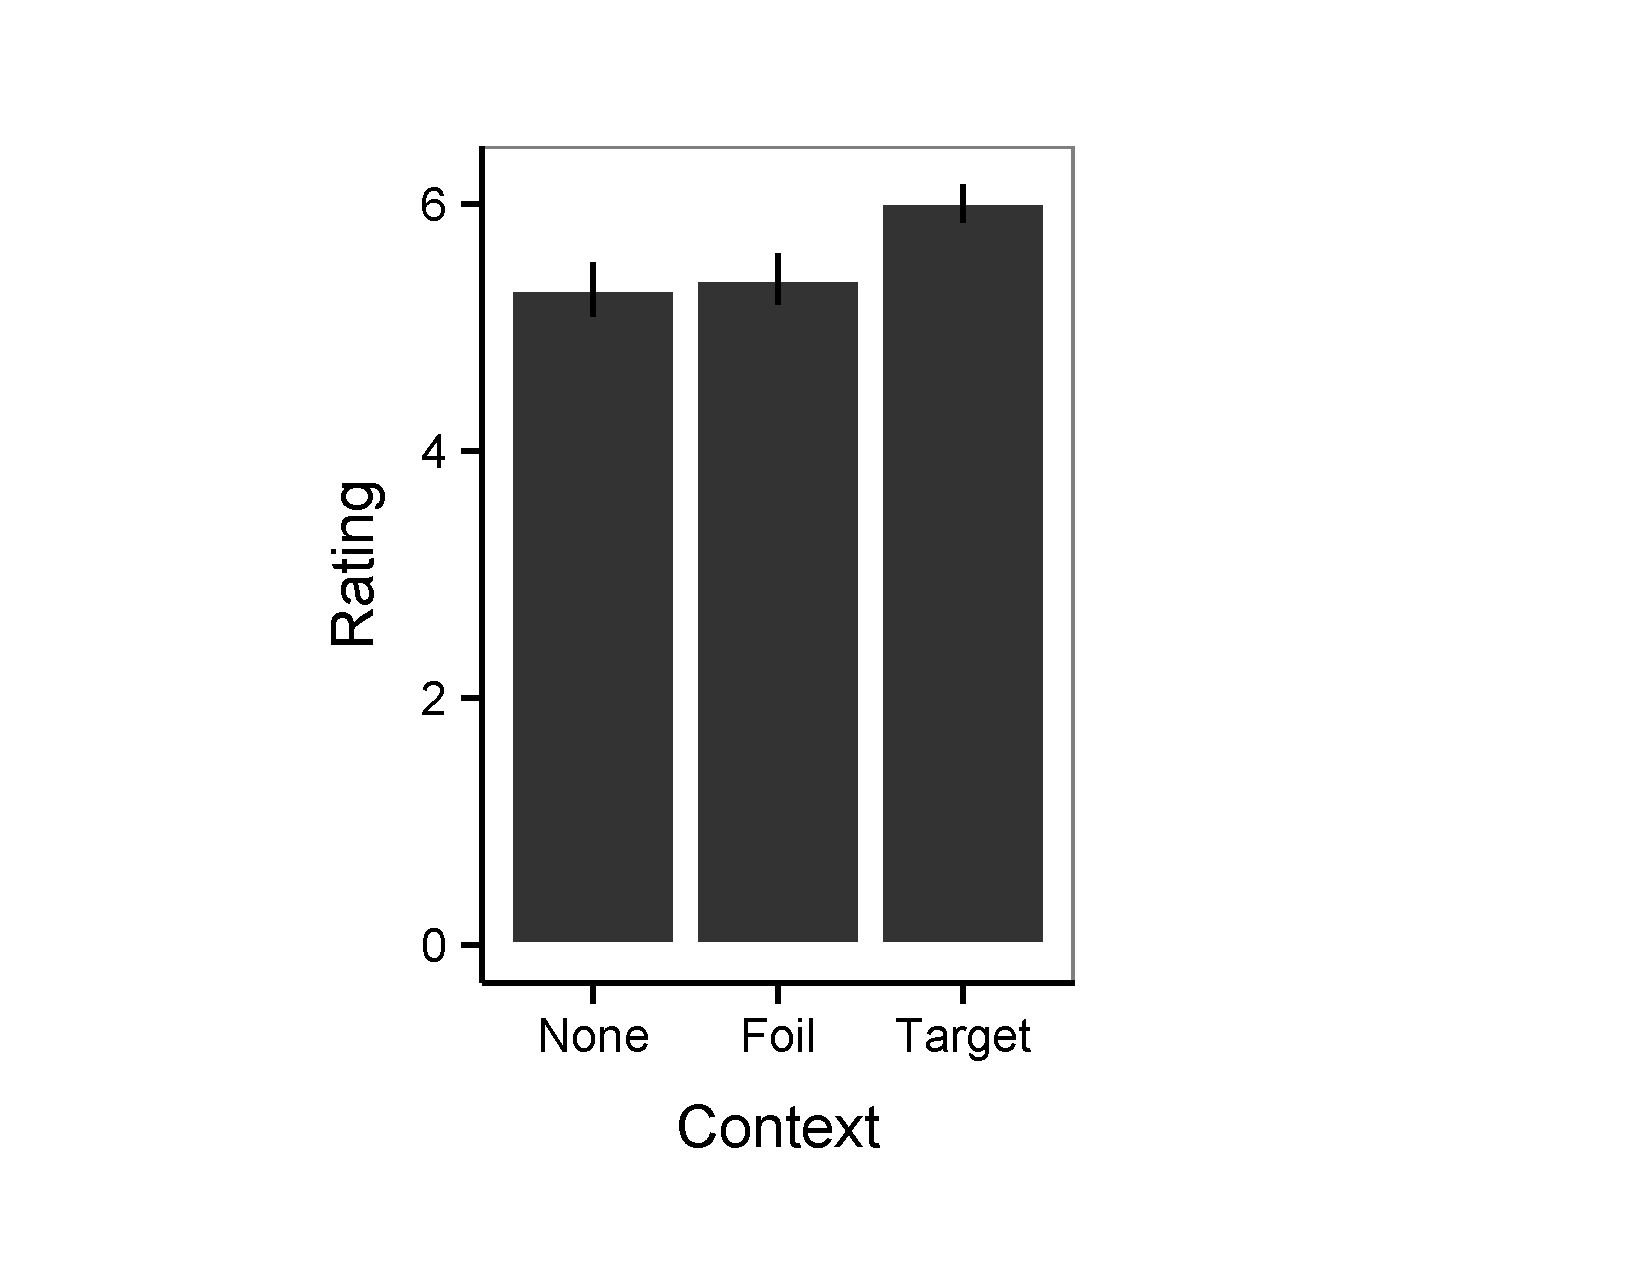
\includegraphics[width=1.8in]{figures/study2.pdf}
\caption{\label{fig:s2} Ratings for true negative sentences in three context conditions in Experiment 2.  Error bars show 95\% confidence intervals.}
\vspace{-1cm}
\end{center} 
\end{figure}

We fit a linear mixed-effects model to true negative sentence ratings to test the effects of context.\footnote{ The model specification was as follows: \texttt{rating $\sim$ context + (1~\textbar~subject) +  (1~\textbar~item)}}  True negative sentences presented in a \emph{target} context received significantly higher ratings than true negative sentences presented in a \emph{none} context ($\beta= .70$, $p< .001$).  There was no significant difference between sentences presented in a \emph{foil} context and sentences presented in a \emph{none} context ($\beta= .09$, $p=.22$).

In Experiment 2, negative sentences were rated as most felicitous in a context where all of the context characters possessed the negated object.  Negative sentences presented in a \emph{foil} context did not differ significantly from negative sentences in a \emph{none} context.  In the foil context, all characters (including the target character) had the same alternative object.  If the pragmatics of negation require the referent of a negative sentence to be the ``odd one out'' (e.g. lacking a feature that everyone else has), we would expect sentences presented in a \emph{foil} context to be rated lower than sentences presented in the \emph{none} context.  The fact that there was no difference between these two contexts suggests that this is not a necessary feature of a supportive pragmatic context for negation.   Instead, negation appears to be pragmatically licensed in contexts where the negative sentence is highly informative.  

\section{Model}

Both of the preceding studies found a significant effect of context on participants' ratings of true negative sentences.  Why does context have this effect on negative sentences?  One hypothesis is that felicity ratings are influenced by the \emph{informativeness} of negative sentences. On theories of pragmatics, speakers should produce sentences that are appropriately informative based on the context.  In a context where most characters have apples and one does not, it is informative to mention the latter character's lack of apples, because this feature is unique to the character being described.

We used a recent probabilistic model of pragmatics to make predictions about participants' felicity ratings, testing this hypothesis. Details of this model---the ``rational speech act'' model of pragmatics---can be found in several previous publications \cite{frank2012,goodman2013,nordmeyer2014}. Here we give a brief sketch of the intuitions behind the model. The probability of a speaker making an utterance in context is defined as being  proportional to the informativeness of the word in context minus its cost.  Informativeness in context is calculated as the number of bits of information conveyed by the utterance.  We assume that the utterance has a uniform probability distribution over its extension in context (e.g., ``doesn't have apples'' applies to any character without apples, leading to a uniform probability of picking out each individual character without apples). We defined cost as the number of words in the utterance multiplied by a cost-per-word parameter; in our simulations, we did not differentiate between different negative sentence frames, and treated negative sentences as having one word more than positive sentences.  Probabilities were normalized over a sparse vocabulary of possible positive or negative utterances that could describe the characters.

\begin{figure}[t]
\begin{center} 
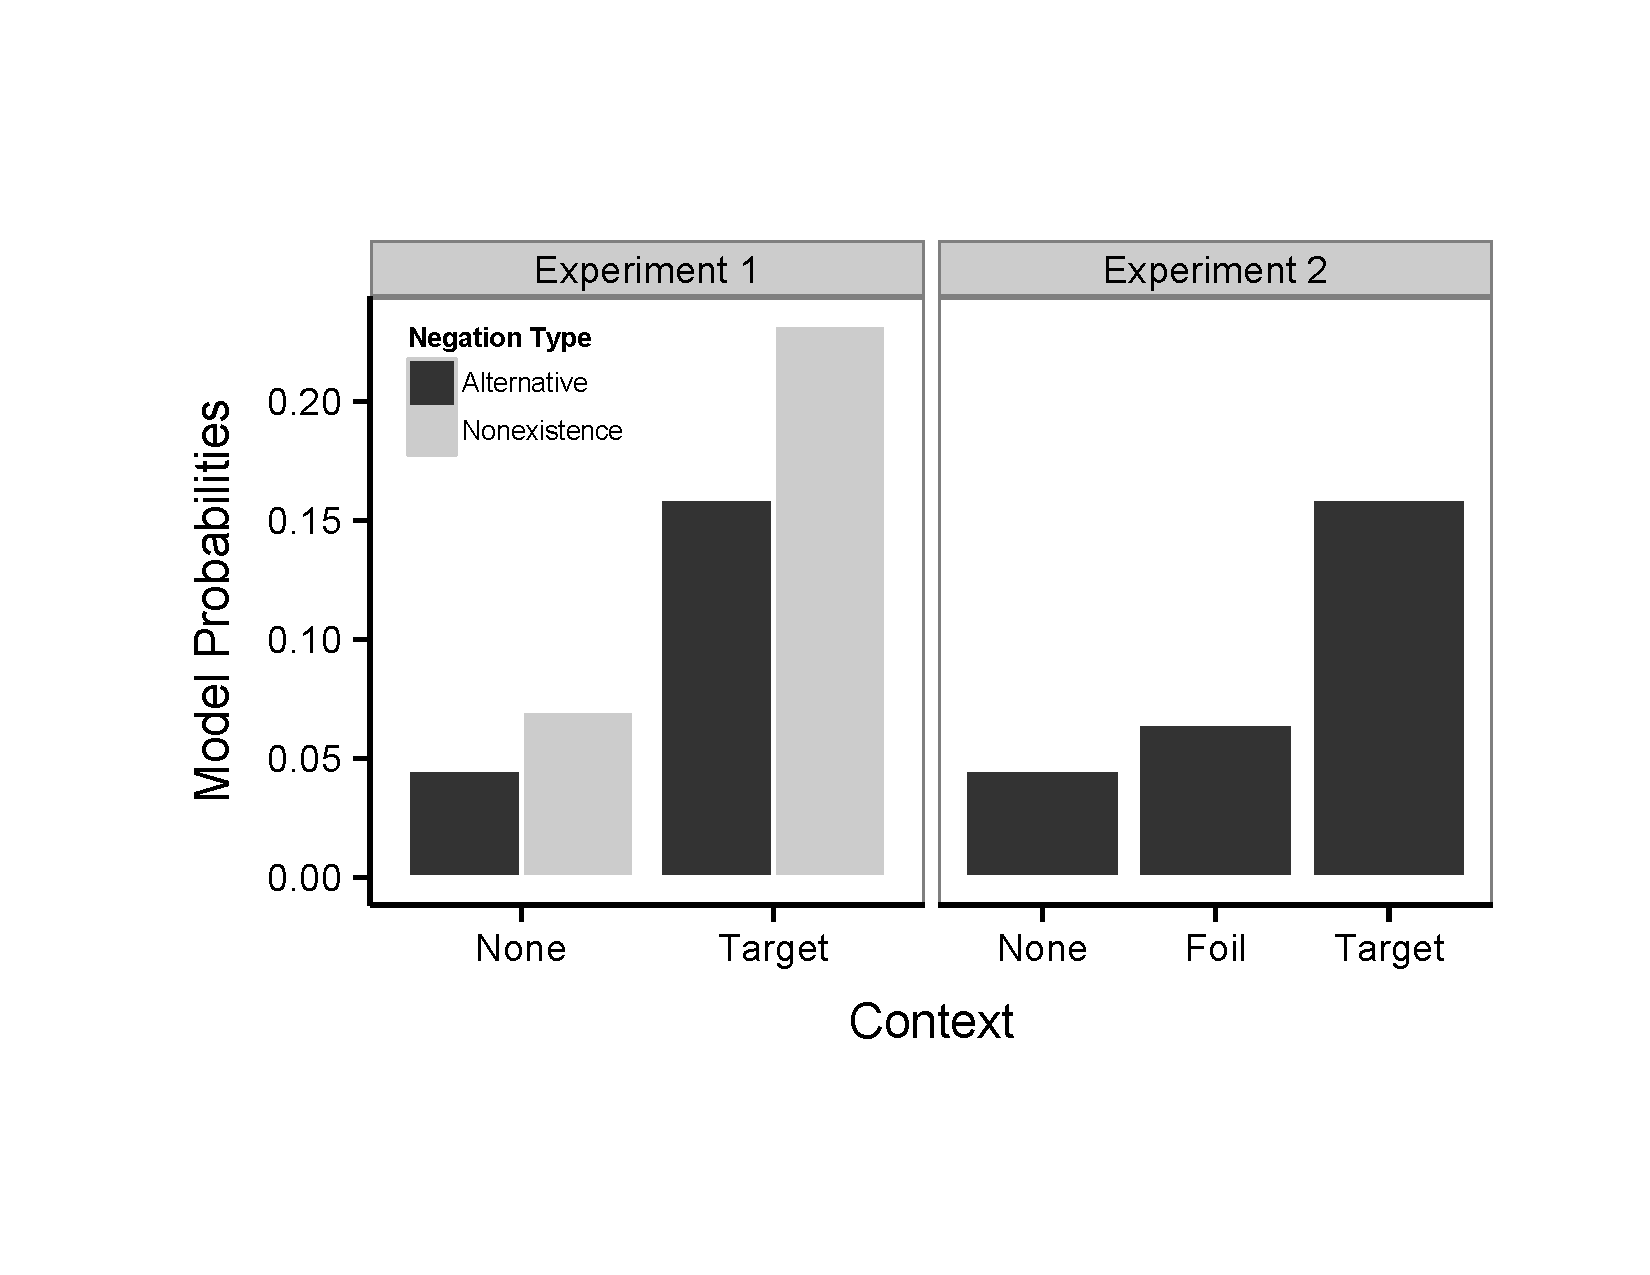
\includegraphics[width=3.25in]{figures/model_predictions.pdf}
\caption{\label{fig:model} Predictions of a model of the informativeness of an utterance in context.  The model predicts how probable a sentence is given a certain context.  Best-fitting parameters were used for this simulation (cost = .8), but the qualitative pattern persists over a wide range of parameter values.  Negative sentences expressing nonexistence are shown in black, and negative sentences referring to an alternative object are shown in gray.}
\vspace{-.2cm}
\end{center} 
\end{figure}

Our model predicted the same qualitative pattern as the data from participants' felicity ratings (Figure \ref{fig:model}).  Sentences presented in a \emph{target} context were preferred over sentences presented in a \emph{none} context, because true negative utterances are more informative when everyone in the context possesses the negated object (e.g., the sentence ``Abby doesn't have an apple'' uniquely identifies Abby when everyone else \emph{does} have apples).  The model predicted that true negatives presented in a \emph{foil} context were more probable than true negatives presented in a \emph{none} context, due to the fact that the positive utterance (e.g. ``Abby has a cat'')  is less informative in the foil context; this difference is not significant in the experimental data.  Nonexistence negation was assigned higher probability than alternative negation, because alternative negation could be described by an equally informative and less costly positive utterance (e.g., ``Abby has a cat'').  Overall, participants' felicity ratings appear to reflect the informativeness of sentences in context.  

\section{Experiment 3}

In Experiment 3, we examined whether children, like adults, find negative sentences more felicitous in informative contexts.  Past work suggests that children produce negation very early \cite{bloom1970, pea1980}, but struggle on classic comprehension tasks for several more years \cite<e.g.>{kim1985}.  Children's success in these tasks is sensitive to the context that a negative sentence occurs in \cite<e.g.>{devilliers1975, nordmeyer2014b}, which could explain this apparent gap between production and comprehension.  If children expect speakers to produce informative utterances, then on classic comprehension tasks they might be reacting to the infelicity of a negative sentence without context rather than its truth value.  Under this account, children should perform differently when they are asked to evaluate negative sentences in a supportive context.  

To simplify the experiment for children, we focused on alternative negation and varied the context (none vs. target) between subjects.  Children were introduced to a puppet who was ``just learning how to talk, and sometimes makes mistakes,'' and were asked to help the puppet learn by indicating on a 5-point smiley face scale whether the puppet's sentence was ``good'' or ``silly or a mistake.''  We deliberately conflated felicity (i.e. ``silliness'') and truth value in order to encourage children to use the negative side of the scale for both incorrect sentences as well as silly sentences.  In past studies using similar paradigms \cite<i.e.>{kim1985}, children treated true negative sentences as ``wrong''; here we evaluate if children are in fact reacting to the (in)felicity of these sentences by comparing their performance in infelicitous contexts (the none condition) to their performance in felicitous contexts (the target condition).

\subsection{Method}

\subsubsection{Participants}

Families visiting Children's Discovery Museum (CDM) in San Jose, CA were invited to participate in this study. Because our mission at CDM is to recruit a diverse sample of families, we used preset criteria for inclusion in the final sample but recruited inclusively regardless of language background.  We also recruited from a broad range of ages, setting a target of 32 included children per age group (three-, and four-year-olds) and ending data collection once this minimum had been reached in all groups after the rejection criteria were applied. In exchange for participation, children were given a sticker and a certificate.

Fourteen children were excluded for being outside the target age range (between three and five years old).  An additional sixteen children were excluded whose parents indicated that they were exposed to English less than 75\% of the time.  One child was excluded for parental interference during the task.  Twelve children declined to continue the experiment after going through the instructions and practice trials, and five additional children were excluded for completing fewer than half of the trials.  

Children who failed to understand the scale, based on their performance on positive sentences, were rejected from the analysis.  Children's responses to true positive sentences were coded as correct if they chose a happy face on the scale (4 or 5), and children's responses to false positive sentences were coded as correct if they chose a sad face on the scale (1 or 2).  Children who chose an incorrect response on more than 2 trials were rejected from analysis.  Eight children were rejected based on this criteria, four three-year-olds and four four-year-olds.   This left a total of 69 children whose data was analyzed: 35 three-year-olds  (mean age = 3;7, range = 3;0 -- 3;11, 20 female and fifteen male) and 34 four-year-olds (mean age = 4;5, range = 4;0 -- 4;11, 17 female and 17 male).  


\subsubsection{Stimuli}

Trials in Experiment 3 had the same structure as trials in the alternative/target and alternative/none conditions of Experiments 1 and 2 (see \ref{fig:trial}), but with only 16 trials.  As in Experiment 2, all negative sentences were of the form ``[character] doesn't have a/an [object].''  Each child evaluated four true positive, two false positive, two false negative, and eight true negative trials.  Context was a between-subjects factor, so with each child viewing trials with either a target context or none context.  

\subsubsection{Procedure}

Parents and children were recruited on the floor of the CDM and were led to a small nearby research room.  Children were invited to sit at a small table in front of an iPad, next to the experimenter.  Parents sat slightly behind their children.  Children were first encouraged to play a short pre-training "dots game" in which children needed to tap a set of five colorful dots in random locations; each dot transformed into an "X" when tapped. This pre-training sequence served both as a filler to engage children while answering any parent questions, and helped children select pictures effectively during the rest of the experiment.

Once this pre-training game was complete, children were introduced to the experimenter's ``puppet friend,'', Furble.  The experimenter told children that Furble was just learning how to talk, and sometimes made mistakes.  Children were then asked if they wanted to play a game that would help the puppet learn.  Once children agreed, the experimenter advanced the iPad to an ``instructions phase.''  During this phase, the experimenter explained that they would look at pictures with Furble, and Furble would say something about one of the pictures.  If the puppet said something ``really good, or right,'' children were told to select the happiest face.  If the puppet said something ``silly, or made a mistake,'' children were told to use the saddest face.  Children were then told to select the slightly happy face if the puppet said something that was ``a little bit good,'' to select the slightly sad face if the puppet said something ``a little bit silly or a little bit of a mistake,'' and to select the neutral face if what the puppet said was ``right in-between.''  After talking about the smiley-face scale, children were given two example trials (a true positive and a false positive), in which the experimenter told the child whether the sentence was good or silly and asked the child to select the corresponding smiley-face.  

Once the children completed the instructions phase, they were given a chance to practice.  The practice consisted of a true positive trial, two false positive trials, and a final true positive trial.  On each trial, the four characters appeared and a red box appeared around the target character.  The smiley-face scale appeared below the characters, and the target sentence was printed at the bottom of the page in small print for the experimenter to read (in the voice of the puppet).  During the practice trials, the experimenter first identified the target character and then encouraged children to look at all of the other characters as well, e.g. ``See Abby?  Here's Abby with all of her friends.  Let's hear what Furble has to say about Abby.''  The puppet would then produce a sentence, and children were asked whether Furble had said something good or silly.  During the practice trials, if children didn't make a response, or made an incorrect response, the experimenter explained the scale again until children made their own response spontaneously.  After these four practice trials, children were asked if they wanted to continue to help the puppet learn, and children who agreed proceeded to the main experiment.

During the main experiment, trials proceeded in the same way as the practice trials, but the experimenter no longer drew children's attention to every context character.  The experimenter would point to the target character and say, ``Here's Abby!  Let's hear what Furble has to say about Abby.'' Children were then encouraged to make a response.  If children produced a word (i.e. ``good'' or ``silly''), but did not make a response, they were reminded again about which face to choose for good or silly sentences.  If children paused for more than five seconds, they were asked if they wanted to hear the sentence again.  After each trial, a star appeared at the top of the screen, serving as a progress bar.  At the end of the experiment, a large smiley face appeared and children were thanked for helping Furble.  

\subsection{Results and Discussion}

As with adults, children rated true sentences significantly higher than false sentences, indicating that the children in this sample were using the scale correctly.  Children's ratings for positive sentences were higher than their ratings for negative sentences, though this is likely due partially to the fact that they were trained on positive sentences and partially to the context effects described below.

Focusing on children's performance on negative sentences, children in the \emph{target} context rated true negative sentences significantly higher than children in the \emph{none} context, supporting our hypothesis that children are sensitive to the felicity of negation in different contexts.  Children rated false negative sentences significantly lower than true negative sentences in both context conditions, suggesting that children in both conditions heard and processed the negation correctly, even when they rated true negative sentences as ``very silly/a mistake'' (see Figure \ref{fig:childmeans}). 

\begin{table}[t]
\caption{\label{tab:m2} Children's mean felicity rating for different trial types in Experiment 3, based on ratings given on a 5-point scale.}
\begin{center}
\small\addtolength{\tabcolsep}{-5pt}
\begin{tabular}{lllrr}
  \hline
  Context & Sentence type & Truth Value &  Mean & Std. Dev. \\ 
  \hline
  None & Positive & True & 4.59  & 0.70\\ 
  None & Positive & False &  1.77 & 1.04\\ 
  None & Negative & True &  2.72 & 1.44 \\ 
  None & Negative & False & 1.96  &1.23 \\ 
  Target & Positive & True &  4.61 & 0.57\\ 
  Target & Positive & False & 1.48  & 0.83 \\ 
  Target & Negative & True & 3.58  & 1.37 \\ 
  Target & Negative & False & 2.18  & 1.38\\ 
   \hline
\end{tabular}
\end{center}
\end{table}

\begin{figure}
\begin{center} 
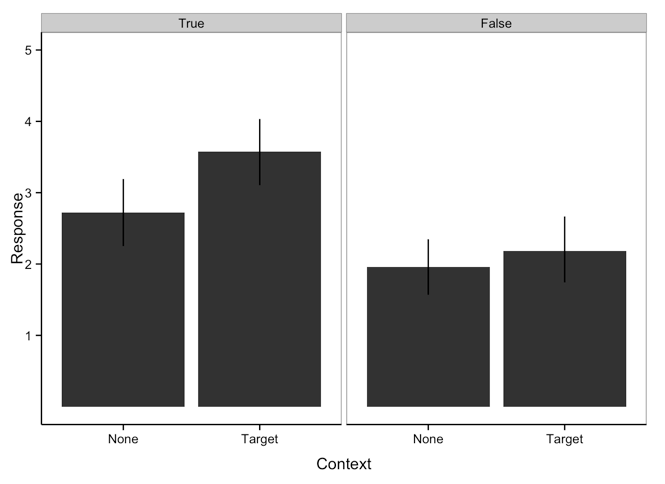
\includegraphics[width=5in]{figures/childmeans.png}
\caption{\label{fig:childmeans} Children's mean ratings for true and false negative sentences in the \emph{none} and \emph{target} contexts in Experiment 3.  Responses to true negatives are shown on the left, and responses to false negatives are shown on the right.  Error bars show 95\% confidence intervals.}
\end{center} 
\end{figure}

We fit a linear mixed-effects model to test the effects of context and truth value on children's negative sentence ratings.\footnote{ The model specification was as follows: \texttt{rating $\sim$ context~$\times$~truth + (1~\textbar~subject) +  (1~\textbar~item)}}   Because children were trained, with feedback, on positive sentences to familiarize them with the scale, and exclusion criteria was based on children's performance on positive sentences, we focus on children's responses to negative sentences in our analyses.  Results of this model can be seen in Table \ref{tab:s3.1}.  Children rated true negative sentences significantly higher than false negative sentences ($\beta= .74$, $p< .001$), indicating that they correctly perceived and processed the negation and recognized that false negative sentences were incorrect.  Although there was no main effect of context on children's responses to negative sentences, a significant interaction between truth value and context indicated that children in the target condition rated true negative sentences significantly higher than did children in the none condition ($\beta= .60$, $p< .05$), supporting our hypothesis that children's past difficulties responding to true negative sentences is due to the infelicity of these sentences, rather than a difficulty in processing negation.  

\begin{table}[t]
\caption{\label{tab:s3.1} Coefficient estimates from a mixed-effects model predicting negative sentence ratings in Experiment 3.}
\begin{center}
\small\addtolength{\tabcolsep}{-5pt}
\begin{tabular}{rrrr}
  \hline
 & Coefficient & Std. err. & t value \\ 
  \hline
(Intercept) & 1.98 & 0.23 & 8.55 \\ 
  Context (target) & 0.25 & 0.33 & 0.74  \\ 
  Truth Value (True) & 0.74 & 0.17 & 4.45 \\
  Context$\times$Truth Value & 0.60 & 0.24 & 2.50 \\
   \hline
\end{tabular}
\end{center}
\end{table}

A linear mixed-effects model that included children's age group did not yield a significant effect of age group (three-year-olds vs. four-year-olds), and did not significantly improve model fit ($\chi ^{2}(4) = 2.35$, $p=.7$).  Figure \ref{fig:histograms} shows histograms of three-year-olds' and four-year-olds' responses to true negative trials, as well as the mean responses to true negative trials in each context condition.  Both three- and four-year-olds were significantly more likely to rate a true negative sentence as ``very good'' in the target condition, and were significantly more likely to rate a true negative sentence as ``very silly / a mistake'' in the none condition.  This effect of context, however, appears to be more pronounced amongst four-year-olds compared to three-year-olds.  To separately examine the effect of context on true negative sentence ratings in each age group, we separately compared each age groups' responses to true negative sentences in the target condition and the none condition.  A two-sample t-test showed that the difference between true negative ratings in the target condition and the none condition was not significant for three-year-olds ($t(32) = -1.56$, $p=0.13$), but was significant for four-year-olds ($t(32) = -2.09$, $p<.05$), indicating that four-year-olds rated true negative sentences significantly lower in the none condition compared to the target condition.  


\begin{figure}
\begin{center} 
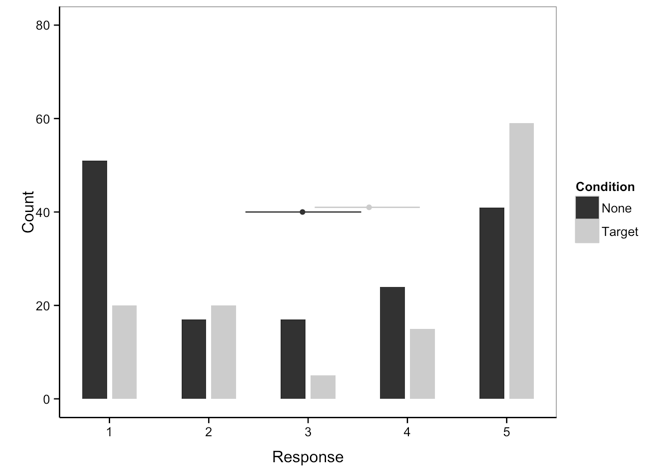
\includegraphics[width=5in]{figures/3hist.png}
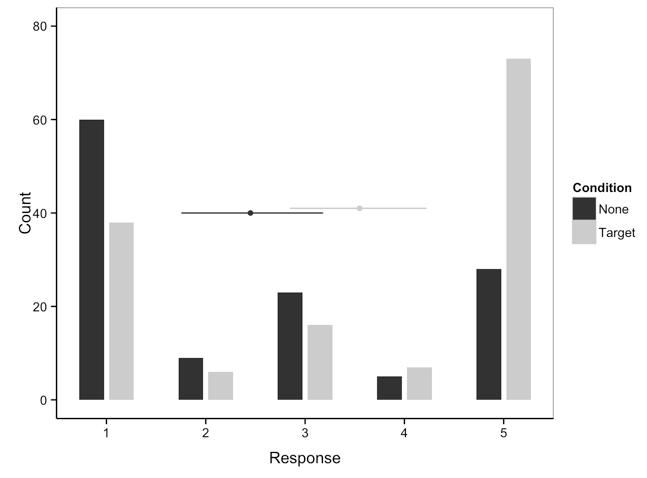
\includegraphics[width=5in]{figures/4hist.png}
\caption{\label{fig:histograms} Histograms of children's responses to true negative trials in the target context and the none context.  3-year-olds are shown above, and 4-year-olds are shown below.  Black bars represent responses in the \emph{none} context, and gray bars represent responses in the \emph{target} context.  Points represent the mean response in each group, and horizontal error bars show 95\% confidence intervals.}
\end{center} 
\end{figure}

%\begin{figure}
%\begin{center} 
%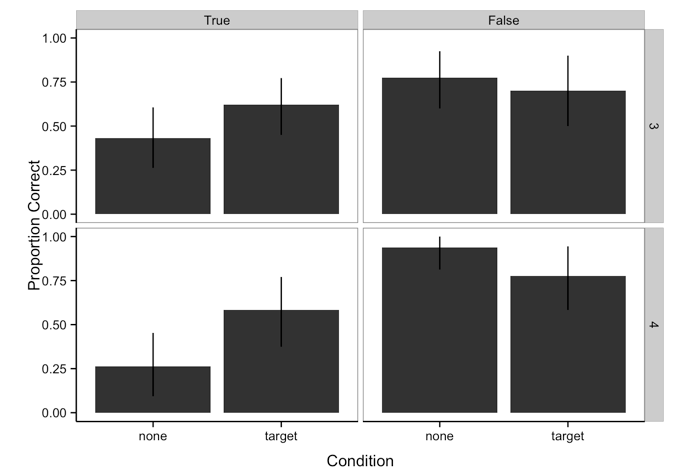
\includegraphics[width=5in]{figures/propcorrect.png}
%\caption{\label{fig:propcorrect} Proportion ``correct'' responses by age, truth value, and condition.  Responses to true negatives were coded as ``correct'' if children chose a happy face (4 or 5), and responses to false negatives were coded as ``correct'' if children chose a sad face (1 or 2).  Three-year-olds are shown above, and four-year-olds are shown below.  Responses to true negatives are on the left, and responses to false negatives are on the right.  }
%\end{center} 
%\end{figure}

%\begin{table}[t]
%\caption{\label{tab:s3.2} Coefficient estimates from a mixed-effects model predicting proportion correct responses to negative sentences in Experiment 3.}
%\begin{center}
%\small\addtolength{\tabcolsep}{-5pt}
%\begin{tabular}{rrrrr}
%  \hline
% & Coefficient & Std. err. & z value & $p|z|$ \\ 
%  \hline
%(Intercept) & 3.37 & 0.68 & 4.99 & $<$.001\\ 
%  Context (target) & -1.31 & 0.82 & -1.60 & 0.11 \\ 
%  Truth Value (True) & -4.27 & 0.57 & -7.55 & $<$.001\\
%  Age group (Four-year-olds) & -0.39 & 0.61 & -0.63 & 0.53 \\
%  Context$\times$Truth Value & 3.15 & 0.69 & 4.55 & $<$.001 \\
%   \hline
%\end{tabular}
%\end{center}
%\end{table}

%(NOTE: I'm feeling ambivalent about whether this is worth including...it feels kind of repetitive?  Also, if I do this here, should I do the same analysis for adults, for the sake of consistency?)
%Although we described our scale as measuring felicity, anchoring the endpoints of the scale at ``good'' vs. ``silly/a mistake'' instead of ``right'' vs. ``wrong'', it is possible to view children's responses as ``correct'' based purely on the truth value of the sentence.  In our adult data, adults nearly always placed even infelicitous true negative sentences on the high side of the scale, and reserved the lower end of the scale for sentences that were overtly false.  We re-coded our data to reflect whether children's responses were ``correct'' based on truth value, with true negatives coded as correct if children chose a happy face on the scale (a 4 or a 5), and false negatives coded as correct if children chose a sad face on the scale (a 1 or a 2).  A plot of mean proportion correct for true and false sentences by context condition and age group is shown in Figure \ref{fig:propcorrect}.   Children in both age groups were significantly more likely to respond to false negative sentences correctly compared to true negative sentences, consistent with the finding that context influences responses to true negative sentences more than it influences responses to false negative sentences.  For true negative sentences, children were significantly more likely to respond correctly to true negative sentences in the target context compared to the none context.  This effect was more pronounced amongst four-year-olds, with four-year-olds' responses to true negatives hovering around floor in the none condition.  

%We fit a binomial mixed-effects model to explore the effects of context, truth value, and age group on correct responses.\footnote{ The model specification was as follows: \texttt{correct $\sim$ context~$\times$~truth~$+$~age.group + (1~\textbar~subject) +  (1~\textbar~item)}} Once again, we did not see a significant main effect of age group ($\beta= .74$, $p< .001$) (NOTE: The model with agegroup as part of a 3-way interaction does not converge, but it does show a marginal effect of age group, and a marginal 3-way interaction.  Should I mention this?  Should I ignore it, because it doesn't converge??)  We found a significant effect of truth value, with children responding correctly to false sentences more often than they responded correctly to true sentences.  We also found a significant interaction between context and truth value, such that children were significantly more likely to respond correctly to true negative sentences in the target condition compared to the none condition.  

Together these results suggest a pronounced effect of context on children's responses to true negative sentences.  Three- and four-year-olds combined rated true negative sentences higher in the target context.  Children did not have difficulty with false negative sentences, suggesting that their performance in response to true negative sentences is not due to confusion about how negation works or difficulty processing negation, but rather a sensitivity to the pragmatics of negation.  Similar to adults, children found true negative sentences to be ``silly'' or a mistake when they were produced in the absence of an informative context, but were more likely to say that the same sentences were ``good'' in an informative context, suggesting that children's responses to these sentences is due to their sensitivity to pragmatics, rather than a difficulty specific to negation.  


\section{General Discussion}

The same negative sentence can sound perfectly fine in one context, but strange in another.  It can refer to \emph{nothing} in one context, but a \emph{difference} in another. In our experiments, we found that contextual differences led to significantly different pragmatic judgments for otherwise identical true grammatical negative sentences.  What is it about the context of negative sentences that elicits these effects?  

The negative sentences that received the lowest felicity ratings for both adults and children were alternative negations in a \emph{none} context.  On these trials, participants saw e.g. three characters with nothing, and a character with a cat (see Figure \ref{fig:trial}).  The sentence ``Abby doesn't have apples'' referred to the character with a cat.  Although this sentence is true, it sounds very odd: Why is the speaker talking about Abby's lack of apples, which is true of everyone in the context, instead of mentioning the cat?  Compare this example to nonexistence negation in a \emph{target} context: Three characters have apples, and Abby has nothing.  Here, the same sentence sounds perfectly natural, because Abby's lack of apples is unique, and there is little else to say about her.  In this latter context, producing a negative sentence is reasonable and perhaps even expected.

Children's responses to negative sentences in the \emph{none} context replicates past findings \cite{kim1985}: Children said that the true negative sentences were ``silly'' or ``a mistake'', despite the fact that the sentences were true.  In contexts where all of the context characters possessed the negated item, however, children's behavior shifted dramatically, with the majority of children rating the true sentences as ``good''.  We can draw two conclusions from children's performance on this task: First, children's past ``failures'' on similar comprehension tasks are likely due to the infelicity of pragmatically unsupported negation.  Instead of interpreting children's responses as ``incorrect'', we can interpret their responses as a felicity judgment: Children in the none condition are saying that the sentence is wrong or a mistake not because it is \emph{false}, but because it is \emph{infelicitous}.  Second, children's performance on this tasks suggests a sensitivity to the contexts of communication more generally.  According to Neo-Gricean theories of communication, speakers should produce sentences that are maximally informative and relevant given the context.  In our experiment, the \emph{none} context was both uninformative and irrelevant.  Children's differential responses to true negative sentences in these two contexts suggests that children are aware of these communicative principles, and expect speakers (and puppets) to abide by them.  

One consistent finding across all three experiments was the effect of context on true negative compared to false negative sentences.  Our primary focus was on true negative sentences, because these have been shown to be influenced by context in the past \cite{wason1965, glenberg1999, nordmeyer2014b} and are the most difficult sentence type in classic sentence verification tasks \cite{hclark1972}.  It is striking to note, however, that in every experiment we found significant effects of context on the evaluation of true negative sentences, but no effect of context on the evaluation of false negative sentences.  It is possible that hearing a false sentence is such a gross violation of the Cooperative Principle that speakers don't consider additional violations, such as an uninformative and irrelevant false sentence.  ((NOTE: I wrote this paragraph because it seemed interesting while I was writing the results...but now that I sat here writing it, I kind of think it is a stupid point, and it's just a floor effect (which is basically what I'm saying, anyway).  It is kind of interesting, though, that in negatron we DO see an effect of context on false sentence, but we don't here?  I'm not sure what to think about that, though.)

According to Grice's Cooperative Principle, speakers should produce utterances that are maximally informative in order to effectively communicate their intentions to a listener.  If listeners expect speakers to abide by this principle, they should prefer sentences that are more informative.  Our results support this view of communication.  Under a model in which the goal of communication is to convey your intended meaning in the most efficient and effective way possible, negative sentences that were more informative (and therefore more likely to be produced by a speaker) were given higher felicity ratings.  These data suggest that general pragmatic factors, rather than some specific quirk of negation, can explain the relative felicity of different negative sentences in context.  


 
 

\bibliographystyle{apacite}

\setlength{\bibleftmargin}{.125in}
\setlength{\bibindent}{-\bibleftmargin}

\bibliography{negation}

\end{document}

